%! TEX root = ../main.tex
\section{Interfaz de Usuario}
\label{sec:res_interfaz}
\observacion{Pruebas preliminares de usabilidad}

En la sección~\ref{sec:interfaz} se describe la prueba de interfaz realizada
durante el desarrollo de \fixme{la solución}{de la UI}, a fin de validar las
hipótesis asumidas y evaluar la usabilidad de la solución.

Esta prueba se divide en dos partes, en la primera, denominada
\emph{Simulación}, los sujetos de prueba utilizan la aplicación, y en la
segunda parte, denominada \emph{Encuesta}, los mismos completan una encuesta
sobre su apreciación de la solución.

\subsection{Simulación}

Las grabaciones realizadas a las sesiones de los usuarios se utilizan para medir
el grado de facilidad de aprendizaje de la interfaz de usuario.

Dados los tres grupo descriptos en~\ref{sec:evaluacion_interfaz_variables}, la
tabla~\ref{tab:interfaz_tiempo_acciones} \fixme{muestra}{tiempo} el tiempo, en segundos,
que le tomo a cada usuario realizar cada una de las acciones la primera vez y
el tiempo que les tomo en promedio las demás veces, para cada una de los grupos
de acciones.

\observacion{Hacer énfasis en la comparación entre el primer y los siguientes}

\begin{table}[!hbt]
\centering
\begin{tabular}{|c|c|c|c|c|c|c|}
\hline
\rowcolor{gris} \textbf{} & \multicolumn{2}{|c|}{\textbf{Menú Contextual}} &
\multicolumn{2}{|c|}{\textbf{Menú de la Interfaz}} &
\multicolumn{2}{|c|}{\textbf{Herramienta}}\\
\hline
\rowcolor{gris} Usuario & Primera & Siguientes & Primera & Siguientes & Primera & Siguientes \\
\hline 1 &  8 &  2.25 &  3 & 9.14 & 11 & 3.0 \\
\hline 2 & 30 &  7.00 &  4 & 3.57 &  7 & 4.5 \\
\hline 3 &  5 &  2.25 &  5 & 1.86 &  1 & 1.0 \\
\hline 4 &  2 & 13.00 &  4 & 2.00 &  1 & 0.5 \\
\hline 5 & 18 &  2.75 &  6 & 4.43 &  6 & 3.0 \\
\hline 6 &  4 & 14.25 & 11 & 7.86 & 13 & 4.0 \\
\hline 7 &  5 &  8.00 &  4 & 4.71 & 20 & 2.5 \\
\hline 8 &  3 &  2.33 & 10 & 3.57 &  3 & 6.5 \\
\hline
\textbf{Promedio} & 9.38 & 6.37 & 5.88 & 4.64 & 7.75 & 3.125 \\
\end{tabular}
\caption{Tiempo por acciones la primera vez y las siguientes veces que se realizo}
\label{tab:interfaz_tiempo_acciones}
\end{table}

En la tabla~\ref{tab:interfaz_tiempo_acciones} se observa consistentemente una
\fixme{mejora}{En relación a qué?} en el tiempo de realización de una acción con
respecto a la primera vez que es realizada. 

\begin{figure}[hbt!]
\centering
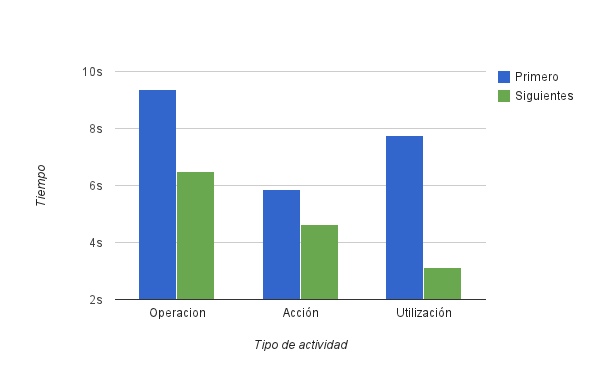
\includegraphics[width=14cm]{resultados/imagenes/interfaz_tiempo_actividades.png}
\caption{Tiempo por tipo de actividad}
\label{fig:interfaz_tiempo_acciones}
\end{figure}

En la figura~\ref{fig:interfaz_tiempo_acciones} se observa como en promedio el
usuario aprende, y en las siguientes acciones similares demora menos tiempo,
este es un factor importante y es el objetivo de esta prueba pues muestra que la
interfaz es fácil de usar, y con tres movimientos básicos, el usuario puede
utilizarla sin mayores inconvenientes. Se observa una mejoría del $30\%$ en las
acciones \emph{Menú Contextual}, $21\%$ en las acciones de tipo \emph{Menú de la
    Interfaz} y finalmente, una mejoría del $60\%$ en las acciones de tipo
\emph{Herramienta}.


La tabla~\ref{tab:interfaz_cantidad_espaciales} nos muestra la cantidad de
movimientos espaciales realizados por los usuarios, se observa que en promedio
se desplazaron $10,88$ veces por el escenario, y $6,75$ veces acercaron o
alejaron la cámara del paciente.

\observacion{Hay que dejar bien en claro de donde sale esto, por que es
importante entender el significado de esta diferencia}

\begin{table}[H]
\centering
\begin{tabular}{lrrr}
\toprule
\textbf{Jugador}  & \textbf{Movimiento} & \textbf{Zoom} & \textbf{Total} \\
\midrule
1        & 18         & 2    & 20 \\
2        & 7          & 8    & 15 \\
3        & 14         & 12   & 26 \\
4        & 9          & 14   & 23 \\
5        & 5          & 8    & 13 \\
6        & 14         & 4    & 18 \\
7        & 16         & 3    & 19 \\
8        & 4          & 3    &  7 \\
\midrule
\textbf{Promedio} & \textbf{10,88}      & \textbf{6,75} & \textbf{17,63} \\
\bottomrule
\end{tabular}
\caption{Cantidad de movimientos espaciales}
\label{tab:interfaz_cantidad_espaciales}
\end{table}

No existe una cantidad mínima o máxima que el usuario debería acercar o mover la
cámara, en cambio, los datos mostrados en~\ref{tab:interfaz_cantidad_espaciales},
muestran que no son necesarias demasiadas acciones, juntando esta información,
con la información proveída en la tabla~\ref{tab:interfaz_tiempo_total}, se ve
que en promedio los usuarios realizaron $1,7$ movimientos por minuto.

\begin{table}[!hbt]
\centering
\begin{tabular}{lrrr}
\toprule
\textbf{Alumno} & \textbf{Tiempo} \\
\midrule
1        & 8:32 \\
2        & 6:03 \\
3        & 8:33 \\
4        & 5:17 \\
5        & 6:55 \\
6        & 8:40 \\
7        & 7:03 \\
8        & 10:27 \\
\midrule
\textbf{Promedio} & \textbf{7:41} \\
\bottomrule
\end{tabular}
\caption{Tiempo de prueba por usuario}
\label{tab:interfaz_tiempo_total}
\end{table}

El tiempo total que se observa en la tabla~\ref{tab:interfaz_tiempo_total},
muestra que en promedio a cada alumno le tomo $7:41$ minutos realizar todos los
pasos especificados, es importante notar que este tiempo incluye el tiempo de
adaptación. 



\begin{table}[!hbt]
\centering
\begin{tabular}{lrrr}
\toprule
\textbf{Alumno} & \textbf{Pasos requeridos} \\
\midrule
1 & 19 \\
2 & 15 \\
3 & 18 \\
4 & 15 \\
5 & 18 \\
6 & 16 \\
7 & 19 \\
8 & 14 \\
\midrule
\textbf{Promedio} & \textbf{16,75} \\
\bottomrule
\end{tabular}
\caption{Acciones realizadas por usuario}
\label{tab:interfaz_acciones}
\end{table}

La tabla~\ref{tab:interfaz_acciones} nos muestra la cantidad de acciones que
realizaron los alumnos, junto con las acciones correctas para llevar a cabo el
procedimiento. Se observa que en promedio realizaron $16.75$ acciones correctas,
esto permite identificar en que parte de procedimiento los usuarios tienen
inconvenientes en cuanto al uso de la interfaz.

\subsection{Encuesta}

\fixme{Como fue descripta en la sección~\ref{sec:interfaz} la encuesta es
realizada a cada usuario}{Mejorar}, y es utilizada para obtener el grado de
disconformidad de los mismos. Se utiliza la disconformidad para resaltar los
puntos débiles, y así, aquellas variables que tengan el mayor porcentaje serán
las que deben ser arregladas.

Las preguntas que forman parte de la  encuesta son agrupadas en cuanto a
aspectos de calidad gráfica, interacción con el entorno, interacción con los
objetos, características del entorno, usabilidad de la interfaz e integración
con el hardware.

Luego de estas agrupaciones obtenemos el resultado que se muestra en la
tabla~\ref{tab:interfaz_disconformidad_metrica}. En esta tabla se puede observar
que las mayores disconformidades son con respecto a la usabilidad de la interfaz
que llega al $51\%$, la interacción de los usuarios con el entorno que llega al
$50\%$, la interacción con los objetos que llega al $49\%$. Luego, se pueden
observar también otras disconformidades con menor porcentaje, las
características del entorno con un  $33\%$, la integración con el hardware con
un  $27\%$ y por ultimo, la calidad gráfica con un  $17\%$.

\observacion{Hay que explicar que estas pruebas se hicieron de forma previa a
las demás y que se arreglan algunos casos}

\begin{table}[H]
\centering
\begin{tabular}{lr}
\toprule
Métrica & Disconformidad \\
\midrule
Calidad Gráfica         & 0.17 \\
Interacción Entorno     & 0.50\\
Interacción Objetos     & 0.49\\
Características Entorno & 0.33\\
Usabililidad Interfaz   & 0.51\\
Integración Hardware    & 0.27\\
\bottomrule
\end{tabular}
\caption{Disconformidad por métrica}
\label{tab:interfaz_disconformidad_metrica}
\end{table}

La conclusión de esta prueba de interfaz, es que si bien, pudo ser utilizada sin
mayores inconvenientes, existe un alto grado de disconformidad con la interfaz,
además cabe resaltar, los sujetos de prueba son personas acostumbradas al uso de
tecnologías similares. Otros puntos débiles encontrados en esta prueba son la
interacción con el entorno y  con los objetos.

Como resultado de esta prueba, la interfaz y la interacción con objetos y
elementos sufren modificaciones a fin de su utilización con usuarios no
técnicos.

Las demás pruebas mencionadas en este capítulo son realizadas con la versión
final de la solución, la cual es obtenida luego de las mejoras realizadas a los
puntos débiles detectados por esta prueba.
